\documentclass{article}
\usepackage{graphicx}
\usepackage{caption}
\usepackage{geometry}
 \geometry{
 a4paper,
 total={170mm,257mm},
 left=20mm,
 top=20mm,
 }
\usepackage{subcaption}
\usepackage{hyperref}
\graphicspath{{./figs/}}{}
\usepackage{listings}
\title{
Rtl-Assignment 9 (PART-2)
}
\begin{document}

\maketitle
\hfill \textbf{RTL-VERILOG}

\section{CRC bits Generator Code}
\begin{figure}[h]
\centering
\begin{subfigure}[b]{0.6\textwidth}
    \centering
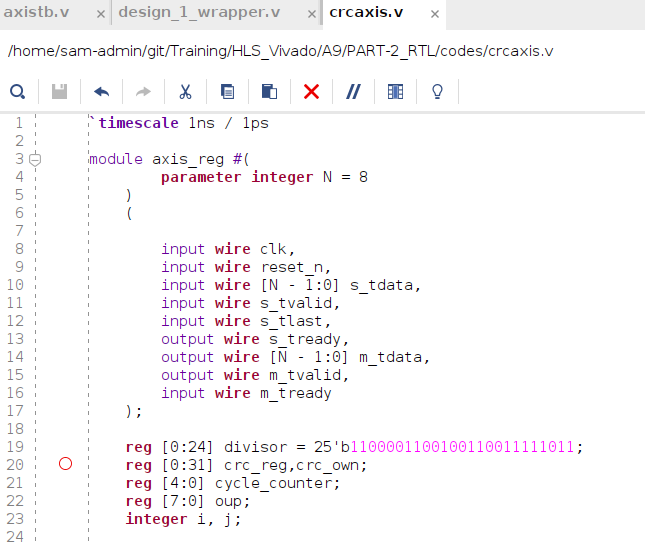
\includegraphics[width=\textwidth]{figs/p2src1.png}
    \label{fig:my_label}
\end{subfigure}
\hfill
\begin{subfigure}[b]{0.6\textwidth}
    \centering
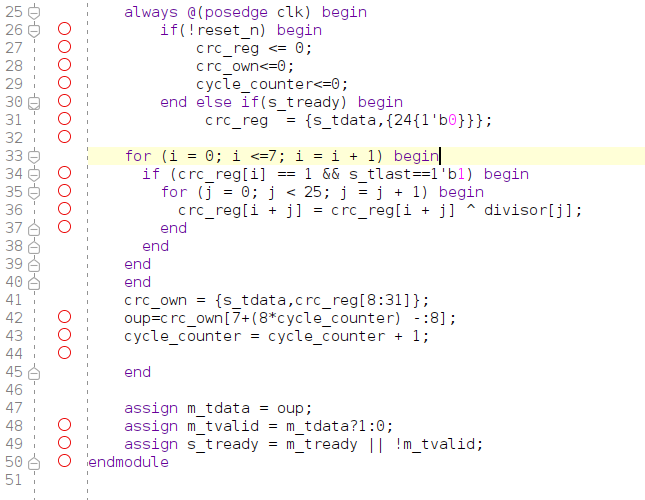
\includegraphics[width=\textwidth]{figs/p2src2.png}
    \caption{crcaxis.v}
    \label{fig:my_label}
\end{subfigure}
\end{figure}

\vspace{13cm}
\section{Design Choices}
\vspace{1cm}
\begin{lstlisting}
1. With same design Choices as PART-1, I designed PART-2 by defining all 
  I/O buses manually.
  
2. s_tdata is the input data,
   s_tvalid indicates the input data validity,
   s_tlast marks the last input data, 
   m_tdata represents the output data, and 
   m_tready represents the activation of port
   m_tvalid indicates the output data validity. 
   The clk and reset_n are clock and reset signals, respectively. 
   The parameter N specifies the width of the data bus.
   
3. the crc_reg is updated by concatenating the input data s_tdata 
  with 24 zeros.
   Same as part-1, here crc_reg performs crc computation and crc_own stores 
  computed data in crc_reg along with input message(s_tdata+crc_reg).
   
   cycle_counter assigns 8 bits of data from crc_own to oup. where, oup is the 
  output data.
   
4. always block sensitive to the positive edge of the clock signal. It handles 
  the CRC calculation. 
   When reset_n is low (active low reset signal), the registers are reset to 
  their initial values.
   When s_tready is high (indicating that the downstream module is ready to 
  accept data), 

5. The two nested for loops are used as followes:
  The outer loop iterates from 0 to 7(to consider only 25 bits of data for 
  computation for inner loop), and 
  The inner loop iterates from 0 to 24.
  It checks if crc_reg[i] is 1 and s_tlast is high (indicating the last input 
  data). If the condition is true, it performs the XOR operation between 
  crc_reg[i + j] and divisor[j], updating the CRC value.

6. After the CRC calculation, the crc_own register is updated by concatenating 
  s_tdata with crc_reg[8:31]. Then, oup is assigned the value of 
  crc_own[7 + (8 * cycle_counter) -: 8], which selects the appropriate 8 bits 
  from crc_own based on the cycle_counter. Finally, the cycle_counter is 
  incremented by 1 to assign next values from crc_own array to oup array.

7. finally, m_tdata is assigned the value of oup, m_tvalid is assigned 1 if 
  m_tdata is non-zero else 0, and s_tready is assigned as m_tready || !m_tvalid. 
  This ensures that s_tready is high when m_tready is high or m_tvalid is low, 
  indicating that the upstream module can send more data.

\end{lstlisting}
\vspace{10cm}
\section{Test Bench Code}
\begin{figure}[h]
\centering
\begin{subfigure}[b]{0.56\textwidth}
    \centering
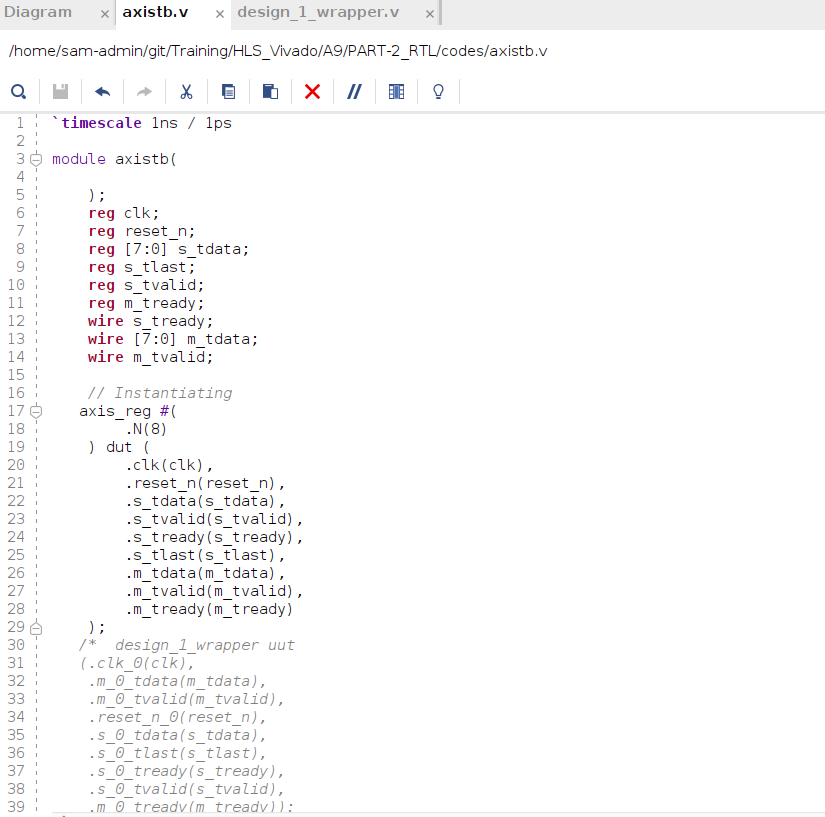
\includegraphics[width=\textwidth]{figs/p2tbrtl1.png}
    \label{fig:my_label}
\end{subfigure}
\hfill
\begin{subfigure}[b]{0.56\textwidth}
    \centering
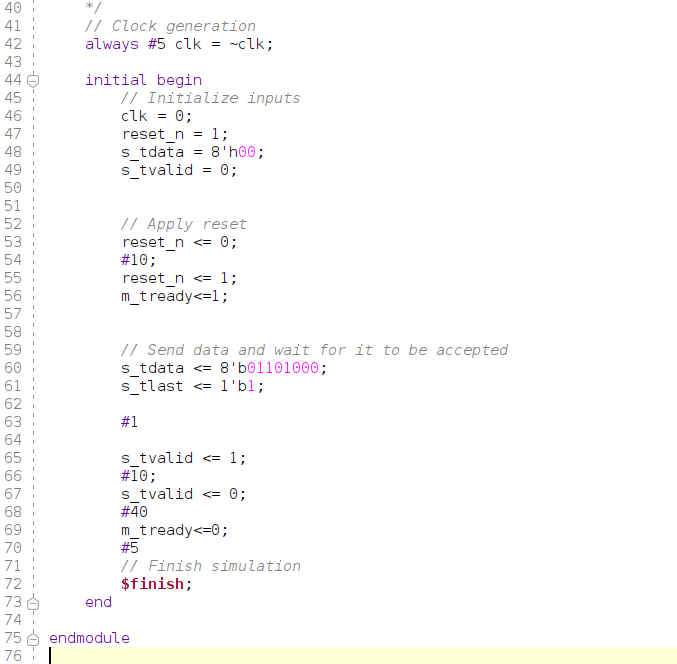
\includegraphics[width=\textwidth]{figs/p2tbrtl2.png}
    \caption{axistb.v}
    \label{fig:my_label}
\end{subfigure}
\end{figure}

\vspace{12cm}

\section{Output Waveform}
\vspace{1cm}
\begin{figure}[h]
    \centering
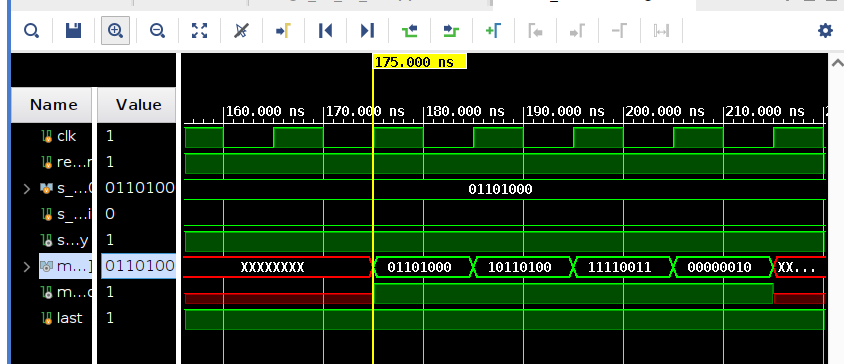
\includegraphics[width=\columnwidth]{figs/p2rtlwav.png}
    \caption{Output of RTL Testbench}
    \label{fig:my_label}
\end{figure}
\vspace{1cm}
\section{Synthesis Report}
\begin{lstlisting}
#-----------------------------------------------------------
# Vivado v2022.2.2 (64-bit)
# SW Build 3788238 on Tue Feb 21 19:59:23 MST 2023
# IP Build 3783773 on Tue Feb 21 23:41:56 MST 2023
# Start of session at: Mon Jul 10 15:25:29 2023
# Process ID: 30364
# Current directory: /home/sam-admin/git/Training/HLS_Vivado/A9/PART-2_RTL/rtl_a9/
rtl_a9.runs/synth_1
# Command line: vivado -log design_1_wrapper.vds -product Vivado -mode batch -
messageDb vivado.pb -notrace -source design_1_wrapper.tcl
# Log file: /home/sam-admin/git/Training/HLS_Vivado/A9/PART-2_RTL/rtl_a9/
rtl_a9.runs/synth_1/design_1_wrapper.vds
# Journal file: /home/sam-admin/git/Training/HLS_Vivado/A9/PART-2_RTL/rtl_a9/
rtl_a9.runs/synth_1/vivado.jou
# Running On: sampaths-lappie, OS: Linux, CPU Frequency: 3398.075 MHz, CPU Physical 
cores: 4, Host memory: 8096 MB
#-----------------------------------------------------------
source design_1_wrapper.tcl -notrace
create_project: Time (s): cpu = 00:00:05 ; elapsed = 00:00:05 . Memory (MB): peak = 
1275.793 ; gain = 0.023 ; free physical = 1794 ; free virtual = 5966
INFO: [IP_Flow 19-234] Refreshing IP repositories
INFO: [IP_Flow 19-1700] Loaded user IP repository '/home/sam-admin/git/Training/
HLS_Vivado/A9/PART-2_RTL/RTL_IP'.
INFO: [IP_Flow 19-2313] Loaded Vivado IP repository '/tools/Xilinx/Vivado/2022.2/
data/ip'.
Command: synth_design -top design_1_wrapper -part xczu7ev-ffvc1156-2-e
Starting synth_design
Attempting to get a license for feature 'Synthesis' and/or device 'xczu7ev'
INFO: [Common 17-349] Got license for feature 'Synthesis' and/or device 'xczu7ev'
INFO: [Device 21-403] Loading part xczu7ev-ffvc1156-2-e
INFO: [Synth 8-7079] Multithreading enabled for synth_design using a maximum of 4 
processes.
INFO: [Synth 8-7078] Launching helper process for spawning children vivado 
processes
INFO: [Synth 8-7075] Helper process launched with PID 30405
INFO: [Synth 8-11241] undeclared symbol 'REGCCE', assumed default net type 
'wire' [/tools/Xilinx/Vivado/2022.2/data/verilog/src/unimacro/BRAM_SINGLE_MACRO.v:
2170]
---------------------------------------------------------------------------------
Starting RTL Elaboration : Time (s): cpu = 00:00:04 ; elapsed = 00:00:05 . Memory 
(MB): peak = 2580.367 ; gain = 241.801 ; free physical = 394 ; free virtual = 4565
Synthesis current peak Physical Memory [PSS] (MB): peak = 2057.646; parent = 
1831.522; children = 226.124
Synthesis current peak Virtual Memory [VSS] (MB): peak = 3578.902; parent = 
2580.371; children = 998.531
---------------------------------------------------------------------------------
INFO: [Synth 8-6157] synthesizing module 'design_1_wrapper' [/home/sam-admin/git/
Training/HLS_Vivado/A9/PART-2_RTL/rtl_a9/rtl_a9.srcs/sources_1/imports/hdl/
design_1_wrapper.v:12]
INFO: [Synth 8-6157] synthesizing module 'design_1' [/home/sam-admin/git/Training/
HLS_Vivado/A9/PART-2_RTL/rtl_a9/rtl_a9.gen/sources_1/bd/design_1/synth/design_1.v:
12]
INFO: [Synth 8-6157] synthesizing module 'design_1_axis_reg_0_0' [/home/sam-admin/
git/Training/HLS_Vivado/A9/PART-2_RTL/rtl_a9/rtl_a9.runs/synth_1/.Xil/Vivado-30364-
sampaths-lappie/realtime/design_1_axis_reg_0_0_stub.v:5]
INFO: [Synth 8-6155] done synthesizing module 'design_1_axis_reg_0_0' (0#1) [/home/
sam-admin/git/Training/HLS_Vivado/A9/PART-2_RTL/rtl_a9/rtl_a9.runs/synth_1/.Xil/
Vivado-30364-sampaths-lappie/realtime/design_1_axis_reg_0_0_stub.v:5]
INFO: [Synth 8-6155] done synthesizing module 'design_1' (0#1) [/home/sam-admin/
git/Training/HLS_Vivado/A9/PART-2_RTL/rtl_a9/rtl_a9.gen/sources_1/bd/design_1/
synth/design_1.v:12]
INFO: [Synth 8-6155] done synthesizing module 'design_1_wrapper' (0#1) [/home/sam-
admin/git/Training/HLS_Vivado/A9/PART-2_RTL/rtl_a9/rtl_a9.srcs/sources_1/imports/
hdl/design_1_wrapper.v:12]
---------------------------------------------------------------------------------
Finished RTL Elaboration : Time (s): cpu = 00:00:06 ; elapsed = 00:00:06 . Memory 
(MB): peak = 2654.336 ; gain = 315.770 ; free physical = 463 ; free virtual = 4636
Synthesis current peak Physical Memory [PSS] (MB): peak = 2057.646; parent = 
1831.522; children = 226.124
Synthesis current peak Virtual Memory [VSS] (MB): peak = 3652.871; parent = 
2654.340; children = 998.531
---------------------------------------------------------------------------------
---------------------------------------------------------------------------------
Start Handling Custom Attributes
---------------------------------------------------------------------------------
---------------------------------------------------------------------------------
Finished Handling Custom Attributes : Time (s): cpu = 00:00:06 ; elapsed = 
00:00:06 . Memory (MB): peak = 2672.148 ; gain = 333.582 ; free physical = 462 ; 
free virtual = 4635
Synthesis current peak Physical Memory [PSS] (MB): peak = 2057.646; parent = 
1831.522; children = 226.124
Synthesis current peak Virtual Memory [VSS] (MB): peak = 3670.684; parent = 
2672.152; children = 998.531
---------------------------------------------------------------------------------
---------------------------------------------------------------------------------
Finished RTL Optimization Phase 1 : Time (s): cpu = 00:00:06 ; elapsed = 00:00:06 . 
Memory (MB): peak = 2672.148 ; gain = 333.582 ; free physical = 462 ; free virtual 
= 4635
Synthesis current peak Physical Memory [PSS] (MB): peak = 2057.646; parent = 
1831.522; children = 226.124
Synthesis current peak Virtual Memory [VSS] (MB): peak = 3670.684; parent = 
2672.152; children = 998.531
---------------------------------------------------------------------------------
Netlist sorting complete. Time (s): cpu = 00:00:00 ; elapsed = 00:00:00 . Memory 
(MB): peak = 2672.148 ; gain = 0.000 ; free physical = 457 ; free virtual = 4629
INFO: [Project 1-570] Preparing netlist for logic optimization

Processing XDC Constraints
Initializing timing engine
Parsing XDC File [/home/sam-admin/git/Training/HLS_Vivado/A9/PART-2_RTL/rtl_a9/
rtl_a9.gen/sources_1/bd/design_1/ip/design_1_axis_reg_0_0/design_1_axis_reg_0_0/
design_1_axis_reg_0_0_in_context.xdc] for cell 'design_1_i/axis_reg_0'
Finished Parsing XDC File [/home/sam-admin/git/Training/HLS_Vivado/A9/PART-2_RTL/
rtl_a9/rtl_a9.gen/sources_1/bd/design_1/ip/design_1_axis_reg_0_0/
design_1_axis_reg_0_0/design_1_axis_reg_0_0_in_context.xdc] for cell 'design_1_i/
axis_reg_0'
Parsing XDC File [/home/sam-admin/git/Training/HLS_Vivado/A9/PART-2_RTL/rtl_a9/
rtl_a9.runs/synth_1/dont_touch.xdc]
Finished Parsing XDC File [/home/sam-admin/git/Training/HLS_Vivado/A9/PART-2_RTL/
rtl_a9/rtl_a9.runs/synth_1/dont_touch.xdc]
Completed Processing XDC Constraints

Netlist sorting complete. Time (s): cpu = 00:00:00 ; elapsed = 00:00:00 . Memory 
(MB): peak = 2756.961 ; gain = 0.000 ; free physical = 403 ; free virtual = 4574
INFO: [Project 1-111] Unisim Transformation Summary:
No Unisim elements were transformed.

Constraint Validation Runtime : Time (s): cpu = 00:00:00 ; elapsed = 00:00:00.01 . 
Memory (MB): peak = 2756.961 ; gain = 0.000 ; free physical = 403 ; free virtual = 
4574
INFO: [Synth 8-11241] undeclared symbol 'REGCCE', assumed default net type 
'wire' [/tools/Xilinx/Vivado/2022.2/data/verilog/src/unimacro/BRAM_SINGLE_MACRO.v:
2170]
---------------------------------------------------------------------------------
Finished Constraint Validation : Time (s): cpu = 00:00:12 ; elapsed = 00:00:13 . 
Memory (MB): peak = 2756.961 ; gain = 418.395 ; free physical = 445 ; free virtual 
= 4619
Synthesis current peak Physical Memory [PSS] (MB): peak = 2059.123; parent = 
1832.999; children = 226.124
Synthesis current peak Virtual Memory [VSS] (MB): peak = 3723.480; parent = 
2724.949; children = 998.531
---------------------------------------------------------------------------------
---------------------------------------------------------------------------------
Start Loading Part and Timing Information
---------------------------------------------------------------------------------
Loading part: xczu7ev-ffvc1156-2-e
INFO: [Synth 8-6742] Reading net delay rules and data
---------------------------------------------------------------------------------
Finished Loading Part and Timing Information : Time (s): cpu = 00:00:12 ; elapsed = 
00:00:13 . Memory (MB): peak = 2756.961 ; gain = 418.395 ; free physical = 445 ; 
free virtual = 4619
Synthesis current peak Physical Memory [PSS] (MB): peak = 2059.123; parent = 
1832.999; children = 226.124
Synthesis current peak Virtual Memory [VSS] (MB): peak = 3723.480; parent = 
2724.949; children = 998.531
---------------------------------------------------------------------------------
---------------------------------------------------------------------------------
Start Applying 'set_property' XDC Constraints
---------------------------------------------------------------------------------
Applied set_property KEEP_HIERARCHY = SOFT for design_1_i. (constraint file  auto 
generated constraint).
Applied set_property KEEP_HIERARCHY = SOFT for design_1_i/axis_reg_0. (constraint 
file  auto generated constraint).
---------------------------------------------------------------------------------
Finished applying 'set_property' XDC Constraints : Time (s): cpu = 00:00:12 ; 
elapsed = 00:00:13 . Memory (MB): peak = 2756.961 ; gain = 418.395 ; free physical 
= 445 ; free virtual = 4619
Synthesis current peak Physical Memory [PSS] (MB): peak = 2059.123; parent = 
1832.999; children = 226.124
Synthesis current peak Virtual Memory [VSS] (MB): peak = 3723.480; parent = 
2724.949; children = 998.531
---------------------------------------------------------------------------------
---------------------------------------------------------------------------------
Finished RTL Optimization Phase 2 : Time (s): cpu = 00:00:12 ; elapsed = 00:00:13 . 
Memory (MB): peak = 2756.961 ; gain = 418.395 ; free physical = 444 ; free virtual 
= 4619
Synthesis current peak Physical Memory [PSS] (MB): peak = 2059.123; parent = 
1832.999; children = 226.124
Synthesis current peak Virtual Memory [VSS] (MB): peak = 3723.480; parent = 
2724.949; children = 998.531
---------------------------------------------------------------------------------
---------------------------------------------------------------------------------
Start RTL Component Statistics 
---------------------------------------------------------------------------------
Detailed RTL Component Info : 
---------------------------------------------------------------------------------
Finished RTL Component Statistics 
---------------------------------------------------------------------------------
---------------------------------------------------------------------------------
Start Part Resource Summary
---------------------------------------------------------------------------------
Part Resources:
DSPs: 1728 (col length:144)
BRAMs: 624 (col length: RAMB18 144 RAMB36 72)
---------------------------------------------------------------------------------
Finished Part Resource Summary
---------------------------------------------------------------------------------
---------------------------------------------------------------------------------
Start Cross Boundary and Area Optimization
---------------------------------------------------------------------------------
WARNING: [Synth 8-7080] Parallel synthesis criteria is not met
---------------------------------------------------------------------------------
Finished Cross Boundary and Area Optimization : Time (s): cpu = 00:00:13 ; elapsed 
= 00:00:15 . Memory (MB): peak = 2756.961 ; gain = 418.395 ; free physical = 417 ; 
free virtual = 4606
Synthesis current peak Physical Memory [PSS] (MB): peak = 2059.123; parent = 
1832.999; children = 226.124
Synthesis current peak Virtual Memory [VSS] (MB): peak = 3723.480; parent = 
2724.949; children = 998.531
---------------------------------------------------------------------------------
---------------------------------------------------------------------------------
Start Applying XDC Timing Constraints
---------------------------------------------------------------------------------
---------------------------------------------------------------------------------
Finished Applying XDC Timing Constraints : Time (s): cpu = 00:00:25 ; elapsed = 
00:00:29 . Memory (MB): peak = 3217.227 ; gain = 878.660 ; free physical = 140 ; 
free virtual = 4044
Synthesis current peak Physical Memory [PSS] (MB): peak = 2621.654; parent = 
2398.049; children = 226.124
Synthesis current peak Virtual Memory [VSS] (MB): peak = 4215.762; parent = 
3217.230; children = 998.531
---------------------------------------------------------------------------------
---------------------------------------------------------------------------------
Start Timing Optimization
---------------------------------------------------------------------------------
---------------------------------------------------------------------------------
Finished Timing Optimization : Time (s): cpu = 00:00:25 ; elapsed = 00:00:29 . 
Memory (MB): peak = 3217.227 ; gain = 878.660 ; free physical = 140 ; free virtual 
= 4044
Synthesis current peak Physical Memory [PSS] (MB): peak = 2621.717; parent = 
2398.111; children = 226.124
Synthesis current peak Virtual Memory [VSS] (MB): peak = 4215.762; parent = 
3217.230; children = 998.531
---------------------------------------------------------------------------------
---------------------------------------------------------------------------------
Start Technology Mapping
---------------------------------------------------------------------------------
---------------------------------------------------------------------------------
Finished Technology Mapping : Time (s): cpu = 00:00:25 ; elapsed = 00:00:29 . 
Memory (MB): peak = 3236.258 ; gain = 897.691 ; free physical = 135 ; free virtual 
= 4037
Synthesis current peak Physical Memory [PSS] (MB): peak = 2622.227; parent = 
2398.633; children = 226.124
Synthesis current peak Virtual Memory [VSS] (MB): peak = 4234.793; parent = 
3236.262; children = 998.531
---------------------------------------------------------------------------------
---------------------------------------------------------------------------------
Start IO Insertion
---------------------------------------------------------------------------------
---------------------------------------------------------------------------------
Start Flattening Before IO Insertion
---------------------------------------------------------------------------------
---------------------------------------------------------------------------------
Finished Flattening Before IO Insertion
---------------------------------------------------------------------------------
---------------------------------------------------------------------------------
Start Final Netlist Cleanup
---------------------------------------------------------------------------------
---------------------------------------------------------------------------------
Finished Final Netlist Cleanup
---------------------------------------------------------------------------------
---------------------------------------------------------------------------------
Finished IO Insertion : Time (s): cpu = 00:00:29 ; elapsed = 00:00:34 . Memory 
(MB): peak = 3242.195 ; gain = 903.629 ; free physical = 133 ; free virtual = 4035
Synthesis current peak Physical Memory [PSS] (MB): peak = 2622.613; parent = 
2399.027; children = 226.124
Synthesis current peak Virtual Memory [VSS] (MB): peak = 4240.730; parent = 
3242.199; children = 998.531
---------------------------------------------------------------------------------
---------------------------------------------------------------------------------
Start Renaming Generated Instances
---------------------------------------------------------------------------------
---------------------------------------------------------------------------------
Finished Renaming Generated Instances : Time (s): cpu = 00:00:29 ; elapsed = 
00:00:34 . Memory (MB): peak = 3242.195 ; gain = 903.629 ; free physical = 133 ; 
free virtual = 4035
Synthesis current peak Physical Memory [PSS] (MB): peak = 2622.629; parent = 
2399.043; children = 226.124
Synthesis current peak Virtual Memory [VSS] (MB): peak = 4240.730; parent = 
3242.199; children = 998.531
---------------------------------------------------------------------------------
---------------------------------------------------------------------------------
Start Rebuilding User Hierarchy
---------------------------------------------------------------------------------
---------------------------------------------------------------------------------
Finished Rebuilding User Hierarchy : Time (s): cpu = 00:00:29 ; elapsed = 
00:00:34 . Memory (MB): peak = 3242.195 ; gain = 903.629 ; free physical = 133 ; 
free virtual = 4035
Synthesis current peak Physical Memory [PSS] (MB): peak = 2622.645; parent = 
2399.059; children = 226.124
Synthesis current peak Virtual Memory [VSS] (MB): peak = 4240.730; parent = 
3242.199; children = 998.531
---------------------------------------------------------------------------------
---------------------------------------------------------------------------------
Start Renaming Generated Ports
---------------------------------------------------------------------------------
---------------------------------------------------------------------------------
Finished Renaming Generated Ports : Time (s): cpu = 00:00:29 ; elapsed = 00:00:34 . 
Memory (MB): peak = 3242.195 ; gain = 903.629 ; free physical = 133 ; free virtual 
= 4035
Synthesis current peak Physical Memory [PSS] (MB): peak = 2622.707; parent = 
2399.121; children = 226.124
Synthesis current peak Virtual Memory [VSS] (MB): peak = 4240.730; parent = 
3242.199; children = 998.531
---------------------------------------------------------------------------------
---------------------------------------------------------------------------------
Start Handling Custom Attributes
---------------------------------------------------------------------------------
---------------------------------------------------------------------------------
Finished Handling Custom Attributes : Time (s): cpu = 00:00:29 ; elapsed = 
00:00:34 . Memory (MB): peak = 3242.195 ; gain = 903.629 ; free physical = 133 ; 
free virtual = 4035
Synthesis current peak Physical Memory [PSS] (MB): peak = 2622.707; parent = 
2399.121; children = 226.124
Synthesis current peak Virtual Memory [VSS] (MB): peak = 4240.730; parent = 
3242.199; children = 998.531
---------------------------------------------------------------------------------
---------------------------------------------------------------------------------
Start Renaming Generated Nets
---------------------------------------------------------------------------------
---------------------------------------------------------------------------------
Finished Renaming Generated Nets : Time (s): cpu = 00:00:29 ; elapsed = 00:00:34 . 
Memory (MB): peak = 3242.195 ; gain = 903.629 ; free physical = 133 ; free virtual 
= 4035
Synthesis current peak Physical Memory [PSS] (MB): peak = 2622.723; parent = 
2399.137; children = 226.124
Synthesis current peak Virtual Memory [VSS] (MB): peak = 4240.730; parent = 
3242.199; children = 998.531
---------------------------------------------------------------------------------
---------------------------------------------------------------------------------
Start Writing Synthesis Report
---------------------------------------------------------------------------------

Report BlackBoxes: 
+------+----------------------+----------+
|      |BlackBox name         |Instances |
+------+----------------------+----------+
|1     |design_1_axis_reg_0_0 |         1|
+------+----------------------+----------+

Report Cell Usage: 
+------+--------------------+------+
|      |Cell                |Count |
+------+--------------------+------+
|1     |design_1_axis_reg_0 |     1|
|2     |IBUF                |    13|
|3     |OBUF                |    10|
+------+--------------------+------+
---------------------------------------------------------------------------------
Finished Writing Synthesis Report : Time (s): cpu = 00:00:29 ; elapsed = 00:00:34 . 
Memory (MB): peak = 3242.195 ; gain = 903.629 ; free physical = 133 ; free virtual 
= 4035
Synthesis current peak Physical Memory [PSS] (MB): peak = 2622.773; parent = 
2399.188; children = 226.124
Synthesis current peak Virtual Memory [VSS] (MB): peak = 4240.730; parent = 
3242.199; children = 998.531
---------------------------------------------------------------------------------
Synthesis finished with 0 errors, 0 critical warnings and 1 warnings.
Synthesis Optimization Runtime : Time (s): cpu = 00:00:27 ; elapsed = 00:00:32 . 
Memory (MB): peak = 3242.195 ; gain = 818.816 ; free physical = 165 ; free virtual 
= 4067
Synthesis Optimization Complete : Time (s): cpu = 00:00:29 ; elapsed = 00:00:34 . 
Memory (MB): peak = 3242.203 ; gain = 903.629 ; free physical = 165 ; free virtual 
= 4066
INFO: [Project 1-571] Translating synthesized netlist
Netlist sorting complete. Time (s): cpu = 00:00:00 ; elapsed = 00:00:00 . Memory 
(MB): peak = 3249.133 ; gain = 0.000 ; free physical = 162 ; free virtual = 4064
INFO: [Netlist 29-17] Analyzing 13 Unisim elements for replacement
INFO: [Netlist 29-28] Unisim Transformation completed in 0 CPU seconds
INFO: [Project 1-570] Preparing netlist for logic optimization
INFO: [Opt 31-138] Pushed 0 inverter(s) to 0 load pin(s).
Netlist sorting complete. Time (s): cpu = 00:00:00 ; elapsed = 00:00:00 . Memory 
(MB): peak = 3275.883 ; gain = 0.000 ; free physical = 204 ; free virtual = 4108
INFO: [Project 1-111] Unisim Transformation Summary:
  A total of 13 instances were transformed.
  IBUF => IBUF (IBUFCTRL, INBUF): 13 instances

Synth Design complete, checksum: 96e7c2a8
INFO: [Common 17-83] Releasing license: Synthesis
26 Infos, 1 Warnings, 0 Critical Warnings and 0 Errors encountered.
synth_design completed successfully
synth_design: Time (s): cpu = 00:00:38 ; elapsed = 00:00:42 . Memory (MB): peak = 
3275.883 ; gain = 1969.121 ; free physical = 400 ; free virtual = 4304
INFO: [Common 17-1381] The checkpoint '/home/sam-admin/git/Training/HLS_Vivado/A9/
PART-2_RTL/rtl_a9/rtl_a9.runs/synth_1/design_1_wrapper.dcp' has been generated.
INFO: [runtcl-4] Executing : report_utilization -file 
design_1_wrapper_utilization_synth.rpt -pb design_1_wrapper_utilization_synth.pb
INFO: [Common 17-206] Exiting Vivado at Mon Jul 10 15:26:23 2023...


\end{lstlisting}

\vspace{1cm}
\section{Resource Utilization}
\begin{lstlisting}
Copyright 1986-2023 Xilinx, Inc. All Rights Reserved.
---------------------------------------------------------------------------------------------------------------------------
| Tool Version : Vivado v.2022.2.2 (lin64) Build 3788238 Tue Feb 21 19:59:23 MST 
2023
| Date         : Mon Jul 10 15:26:23 2023
| Host         : sampaths-lappie running 64-bit Ubuntu 22.04.2 LTS
| Command      : report_utilization -file design_1_wrapper_utilization_synth.rpt -
pb design_1_wrapper_utilization_synth.pb
| Design       : design_1_wrapper
| Device       : xczu7ev-ffvc1156-2-e
| Speed File   : -2
| Design State : Synthesized
---------------------------------------------------------------------------------------------------------------------------

Utilization Design Information

Table of Contents
-----------------
1. CLB Logic
1.1 Summary of Registers by Type
2. BLOCKRAM
3. ARITHMETIC
4. I/O
5. CLOCK
6. ADVANCED
7. CONFIGURATION
8. Primitives
9. Black Boxes
10. Instantiated Netlists

1. CLB Logic
------------

+-------------------------+------+-------+------------+-----------+-------+
|        Site Type        | Used | Fixed | Prohibited | Available | Util% |
+-------------------------+------+-------+------------+-----------+-------+
| CLB LUTs*               |    0 |     0 |          0 |    230400 |  0.00 |
|   LUT as Logic          |    0 |     0 |          0 |    230400 |  0.00 |
|   LUT as Memory         |    0 |     0 |          0 |    101760 |  0.00 |
| CLB Registers           |    0 |     0 |          0 |    460800 |  0.00 |
|   Register as Flip Flop |    0 |     0 |          0 |    460800 |  0.00 |
|   Register as Latch     |    0 |     0 |          0 |    460800 |  0.00 |
| CARRY8                  |    0 |     0 |          0 |     28800 |  0.00 |
| F7 Muxes                |    0 |     0 |          0 |    115200 |  0.00 |
| F8 Muxes                |    0 |     0 |          0 |     57600 |  0.00 |
| F9 Muxes                |    0 |     0 |          0 |     28800 |  0.00 |
+-------------------------+------+-------+------------+-----------+-------+
* Warning! The Final LUT count, after physical optimizations and full 
implementation, is typically lower. Run opt_design after synthesis, if not already 
completed, for a more realistic count.
Warning! LUT value is adjusted to account for LUT combining.


1.1 Summary of Registers by Type
--------------------------------

+-------+--------------+-------------+--------------+
| Total | Clock Enable | Synchronous | Asynchronous |
+-------+--------------+-------------+--------------+
| 0     |            _ |           - |            - |
| 0     |            _ |           - |          Set |
| 0     |            _ |           - |        Reset |
| 0     |            _ |         Set |            - |
| 0     |            _ |       Reset |            - |
| 0     |          Yes |           - |            - |
| 0     |          Yes |           - |          Set |
| 0     |          Yes |           - |        Reset |
| 0     |          Yes |         Set |            - |
| 0     |          Yes |       Reset |            - |
+-------+--------------+-------------+--------------+


2. BLOCKRAM
-----------

+----------------+------+-------+------------+-----------+-------+
|    Site Type   | Used | Fixed | Prohibited | Available | Util% |
+----------------+------+-------+------------+-----------+-------+
| Block RAM Tile |    0 |     0 |          0 |       312 |  0.00 |
|   RAMB36/FIFO* |    0 |     0 |          0 |       312 |  0.00 |
|   RAMB18       |    0 |     0 |          0 |       624 |  0.00 |
| URAM           |    0 |     0 |          0 |        96 |  0.00 |
+----------------+------+-------+------------+-----------+-------+
* Note: Each Block RAM Tile only has one FIFO logic available and therefore can 
accommodate only one FIFO36E2 or one FIFO18E2. However, if a FIFO18E2 occupies a 
Block RAM Tile, that tile can still accommodate a RAMB18E2


3. ARITHMETIC
-------------

+-----------+------+-------+------------+-----------+-------+
| Site Type | Used | Fixed | Prohibited | Available | Util% |
+-----------+------+-------+------------+-----------+-------+
| DSPs      |    0 |     0 |          0 |      1728 |  0.00 |
+-----------+------+-------+------------+-----------+-------+


4. I/O
------

+------------+------+-------+------------+-----------+-------+
|  Site Type | Used | Fixed | Prohibited | Available | Util% |
+------------+------+-------+------------+-----------+-------+
| Bonded IOB |   23 |     0 |          0 |       360 |  6.39 |
+------------+------+-------+------------+-----------+-------+


5. CLOCK
--------

+----------------------+------+-------+------------+-----------+-------+
|       Site Type      | Used | Fixed | Prohibited | Available | Util% |
+----------------------+------+-------+------------+-----------+-------+
| GLOBAL CLOCK BUFFERs |    0 |     0 |          0 |       544 |  0.00 |
|   BUFGCE             |    0 |     0 |          0 |       208 |  0.00 |
|   BUFGCE_DIV         |    0 |     0 |          0 |        32 |  0.00 |
|   BUFG_GT            |    0 |     0 |          0 |       144 |  0.00 |
|   BUFG_PS            |    0 |     0 |          0 |        96 |  0.00 |
|   BUFGCTRL*          |    0 |     0 |          0 |        64 |  0.00 |
| PLL                  |    0 |     0 |          0 |        16 |  0.00 |
| MMCM                 |    0 |     0 |          0 |         8 |  0.00 |
+----------------------+------+-------+------------+-----------+-------+
* Note: Each used BUFGCTRL counts as two GLOBAL CLOCK BUFFERs. This table does not 
include global clocking resources, only buffer cell usage. See the Clock 
Utilization Report (report_clock_utilization) for detailed accounting of global 
clocking resource availability.


6. ADVANCED
-----------

+-----------------+------+-------+------------+-----------+-------+
|    Site Type    | Used | Fixed | Prohibited | Available | Util% |
+-----------------+------+-------+------------+-----------+-------+
| GTHE4_CHANNEL   |    0 |     0 |          0 |        20 |  0.00 |
| GTHE4_COMMON    |    0 |     0 |          0 |         5 |  0.00 |
| OBUFDS_GTE4     |    0 |     0 |          0 |        10 |  0.00 |
| OBUFDS_GTE4_ADV |    0 |     0 |          0 |        10 |  0.00 |
| PCIE40E4        |    0 |     0 |          0 |         2 |  0.00 |
| PS8             |    0 |     0 |          0 |         1 |  0.00 |
| SYSMONE4        |    0 |     0 |          0 |         1 |  0.00 |
| VCU             |    0 |     0 |          0 |         1 |  0.00 |
+-----------------+------+-------+------------+-----------+-------+


7. CONFIGURATION
----------------

+-------------+------+-------+------------+-----------+-------+
|  Site Type  | Used | Fixed | Prohibited | Available | Util% |
+-------------+------+-------+------------+-----------+-------+
| BSCANE2     |    0 |     0 |          0 |         4 |  0.00 |
| DNA_PORTE2  |    0 |     0 |          0 |         1 |  0.00 |
| EFUSE_USR   |    0 |     0 |          0 |         1 |  0.00 |
| FRAME_ECCE4 |    0 |     0 |          0 |         1 |  0.00 |
| ICAPE3      |    0 |     0 |          0 |         2 |  0.00 |
| MASTER_JTAG |    0 |     0 |          0 |         1 |  0.00 |
| STARTUPE3   |    0 |     0 |          0 |         1 |  0.00 |
+-------------+------+-------+------------+-----------+-------+


8. Primitives
-------------

+----------+------+---------------------+
| Ref Name | Used | Functional Category |
+----------+------+---------------------+
| INBUF    |   13 |                 I/O |
| IBUFCTRL |   13 |              Others |
| OBUF     |   10 |                 I/O |
+----------+------+---------------------+


9. Black Boxes
--------------

+-----------------------+------+
|        Ref Name       | Used |
+-----------------------+------+
| design_1_axis_reg_0_0 |    1 |
+-----------------------+------+


\end{lstlisting}
\vspace{12cm}


\maketitle
\hfill \textbf{VIVADO-IP}
\section{Block Design}
\vspace{1cm}
\begin{figure}[h]
    \centering
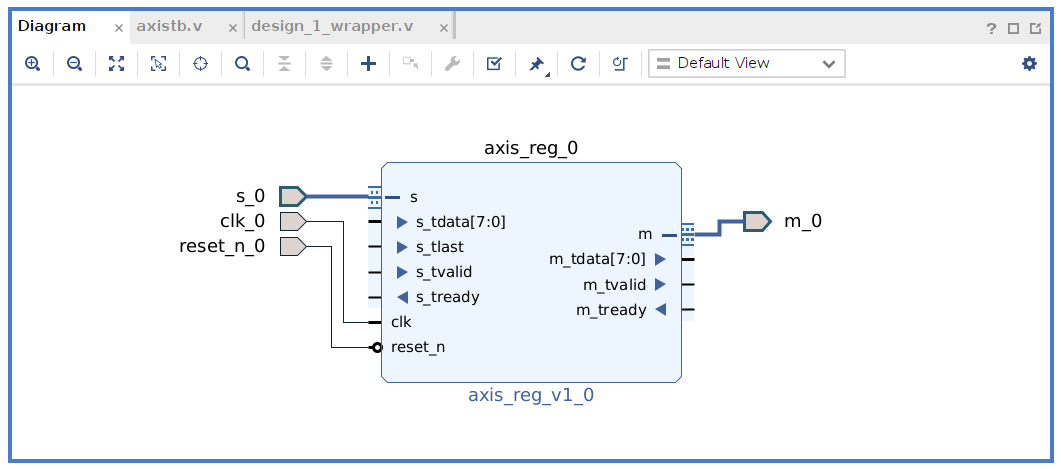
\includegraphics[width=\columnwidth]{figs/p2bd.png}
    \caption{Block Diagram}
    \label{fig:my_label}
\end{figure}
\vspace{13cm}

\section{Verilog Testbench}
\begin{figure}[h]
\centering
\begin{subfigure}[b]{0.6\textwidth}
    \centering
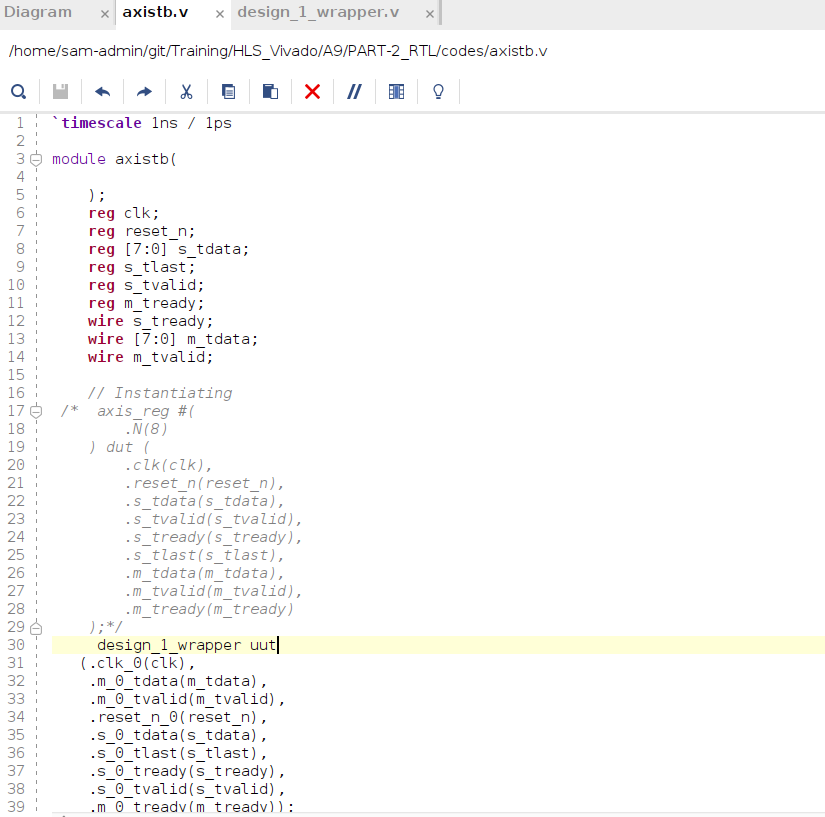
\includegraphics[width=\textwidth]{figs/p2tbip1.png}
    \label{fig:my_label}
\end{subfigure}
\hfill
\begin{subfigure}[b]{0.6\textwidth}
    \centering
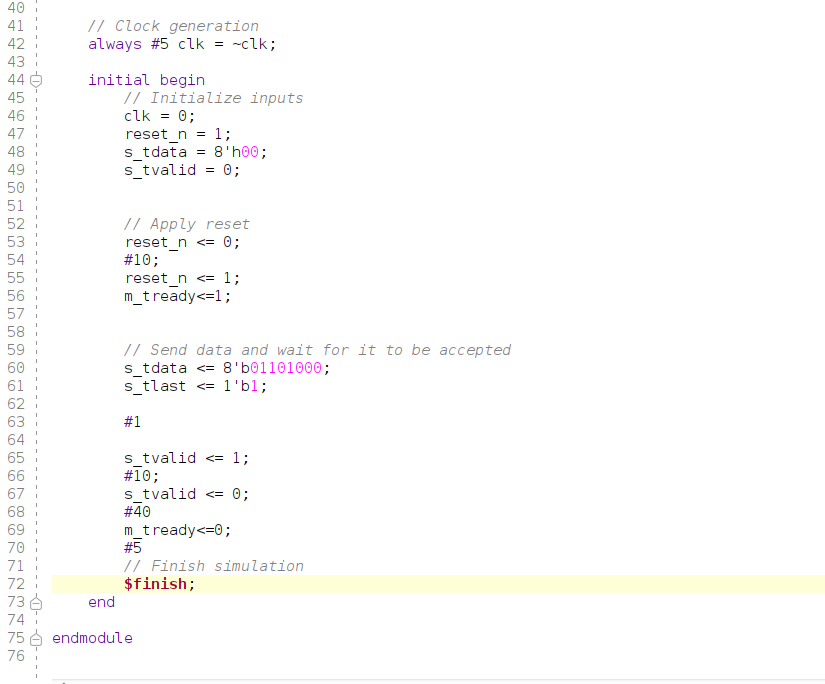
\includegraphics[width=\textwidth]{figs/p2tbip2.png}
    \caption{axistb.v}
    \label{fig:my_label}
\end{subfigure}
\end{figure}

\vspace{13cm}


\section{Output Waveform}
\vspace{1cm}
\begin{figure}[h]
    \centering
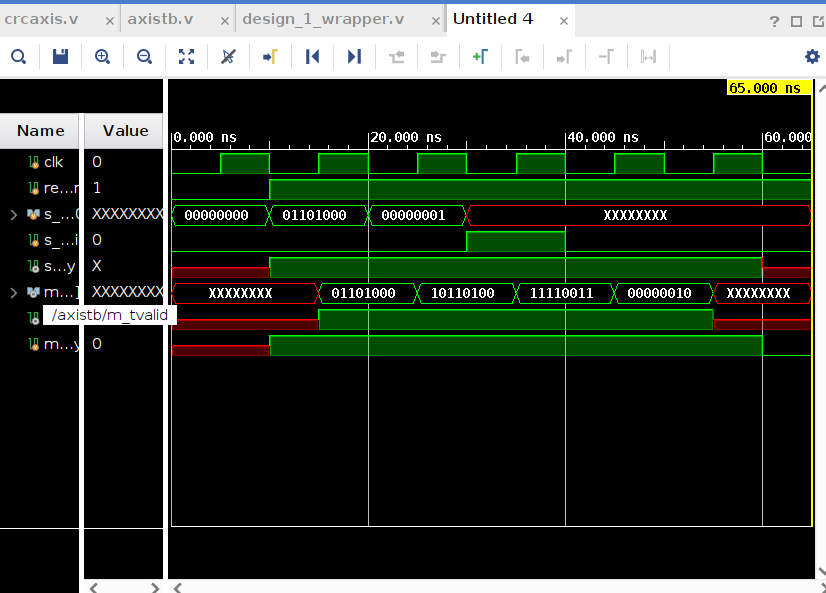
\includegraphics[width=\columnwidth]{figs/p2ipwav.png}
    \caption{Output of IP Testbench}
    \label{fig:my_label}
\end{figure}

\vspace{1cm}

\maketitle
\hfill \textbf{MATLAB REFERENCE}
\section{Matlab Reference}
\begin{figure}[h]
\centering
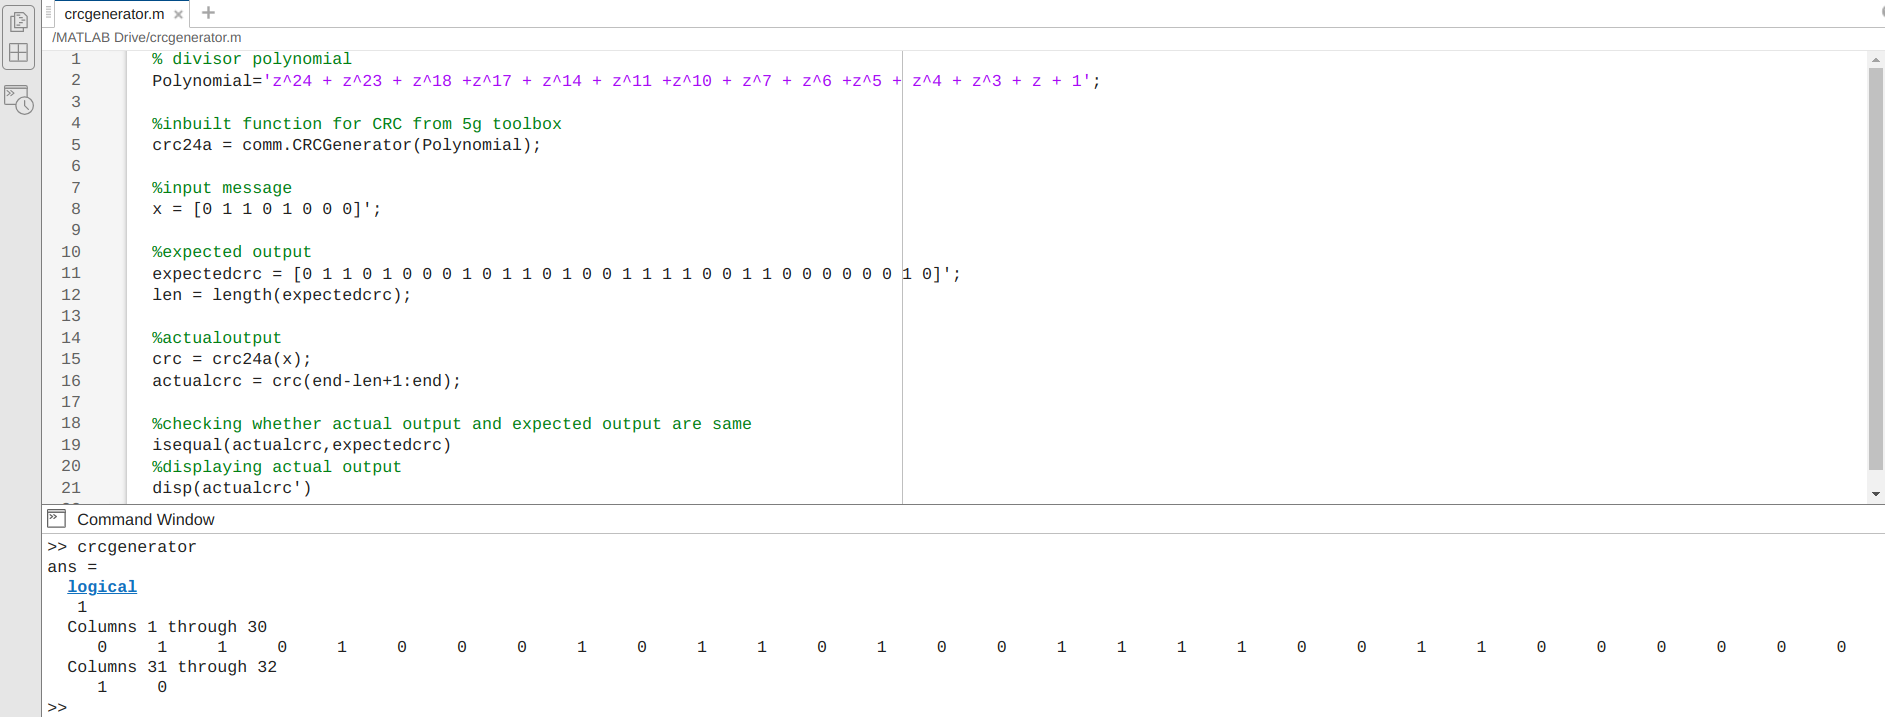
\includegraphics[width=1.1\textwidth]{figs/actual_matlab.png}
    \caption{Matlab Reference}
    \label{fig:my_label}
\end{figure}
\vspace{3cm}
\section{Conclusion}
\begin{lstlisting}
The Output of CRC IP in both PART-1 and Part-2 is matching with Output of 
reference Matlab code and also using this floating Point Converter Online :

\end{lstlisting}
\url{https://www.h-schmidt.net/FloatConverter/IEEE754.html}
\vspace{2cm}
\\
\textbf{GITHUB :} \url{https://github.com/dk-425/Training.git}
\end{document}


